\documentclass{beamer}
\usetheme{default}
\graphicspath{ {imagenes/} }
\usepackage{graphicx}
\usepackage{eurosym}
\usepackage{subfig}

\title{Sistema de adaptación motora con entorno de realidad virtual}
\author{Celia Arias Martínez}
\begin{document}
\begin{frame}[plain]
    \maketitle
\end{frame}



\begin{frame}{}
	\frametitle{Índice}
	\tableofcontents
\end{frame}


\section{Introducción}
\subsection{Estado del arte}

\begin{frame}
	\frametitle{Estado del arte}

\end{frame}
\subsection{Objetivos}

\begin{frame}
\frametitle{Objetivos}
\begin{itemize}
	\item Objetivos técnicos
	\begin{enumerate}
		\item Analizar cómo los dispositivos hápticos (en concreto \textit{3DSystems Touch}) pueden utilizarse en el estudio de movimientos balísticos.
		\item Estudiar la precisión de los datos obtenidos con el dispositivo \textit{Touch}.
		\item Interpretar dichos datos.
	\end{enumerate}
	\item Objetivos didáctivos
	\begin{enumerate}
		\item Aprender a usar \textit{3DSystems Touch}.
		\item Desarrollar una aplicación utilizando la API de \textit{Touch}.
		\item Entender algunas de las aplicaciones de la Geometría a la Informática Gráfica.
		\item Llevar a cabo una experimentación con diferentes sujetos.
		\item Realizar un análisis de los datos obtenidos.
	\end{enumerate}
\end{itemize}

\end{frame}
\subsection{Fases del proyecto}
\begin{frame}
\frametitle{Fases del proyecto}	
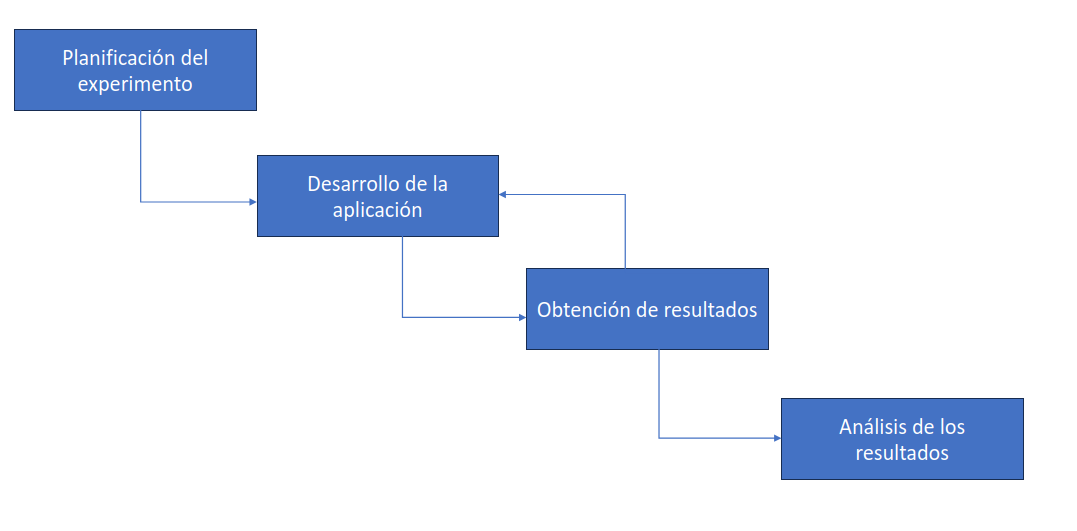
\includegraphics[width=\linewidth]{diagrama-fases}
\begin{itemize}
	\item Modelo de ciclo de vida en \textbf{cascada con realimentación}
\end{itemize}

\end{frame}

\subsection{Planificación del proyecto}

\begin{frame}
\frametitle{Planificación}


\begin{enumerate}
	\item Septiembre: Estudio del estado del arte y planificación
	\item De octubre a noviembre: desarrollo de la aplicación
	\item De enero a marzo: obtención de resultados
	\item De marzo a mayo: análisis de resultados y redacción
\end{enumerate}
\begin{figure}
	\centering
	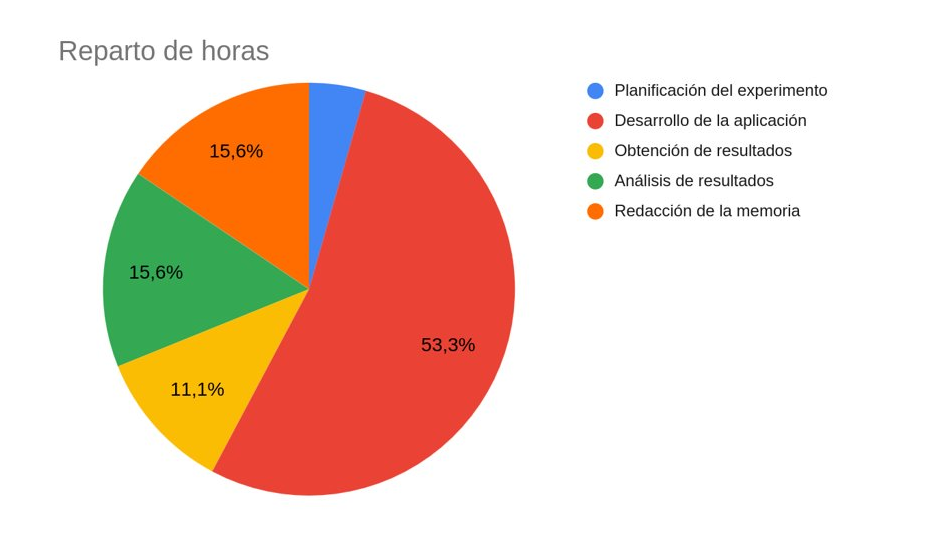
\includegraphics[width=0.8\textwidth]{horas}
\end{figure}


\end{frame}

\begin{frame}
\frametitle{Planificación}
	
\begin{enumerate}
	\item Contratación personal: 9000\euro
	\item Material: 3000\euro
	\item Desarrollo del experimento: 130\euro
\end{enumerate}	
	
\begin{figure}
	\centering
	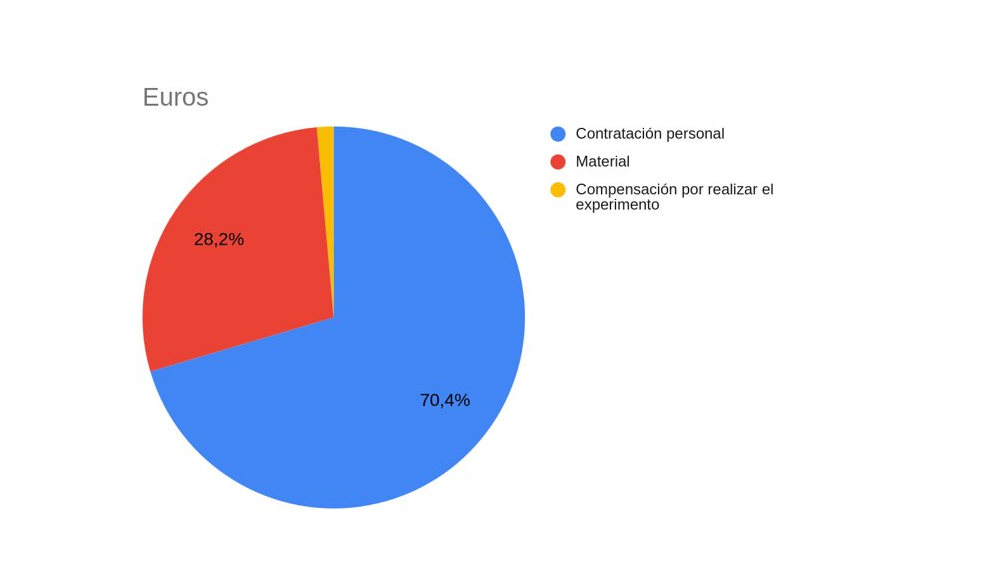
\includegraphics[width=0.8\textwidth]{coste}
\end{figure}
	
\end{frame}

\subsection{Material}

\begin{frame}
	\frametitle{3D Systems Touch y OpenHaptics}
	
\begin{figure}
	\centering
	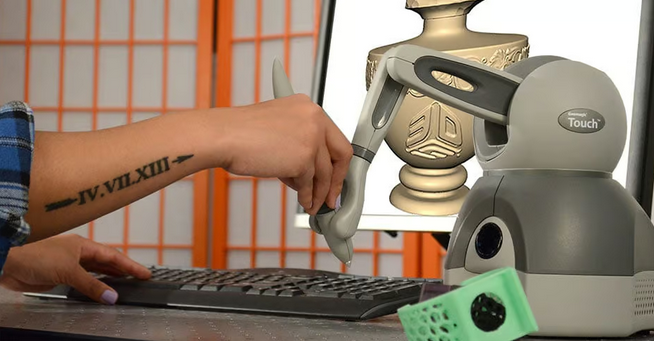
\includegraphics[width=0.8\textwidth]{touch}
\end{figure}
	
Dispositivo háptico desarrollado por \textbf{3D Systems} para simular objetos virtuales a medida que el usuario manipula objetos 3D en la pantalla.
\begin{itemize}
	\item Control robótico
	\item Medicina y cirugía
	\item Rehabilitación, etc.
\end{itemize}		
\end{frame}

\section{Fundamentos matemáticos}

\section{Implementación del proyecto}
\subsection{Planificación del experimento}
\begin{frame}
	\frametitle{Planificación del experimento}
	\fontsize{8pt}{9pt}\selectfont
	\begin{figure}
		\centering
		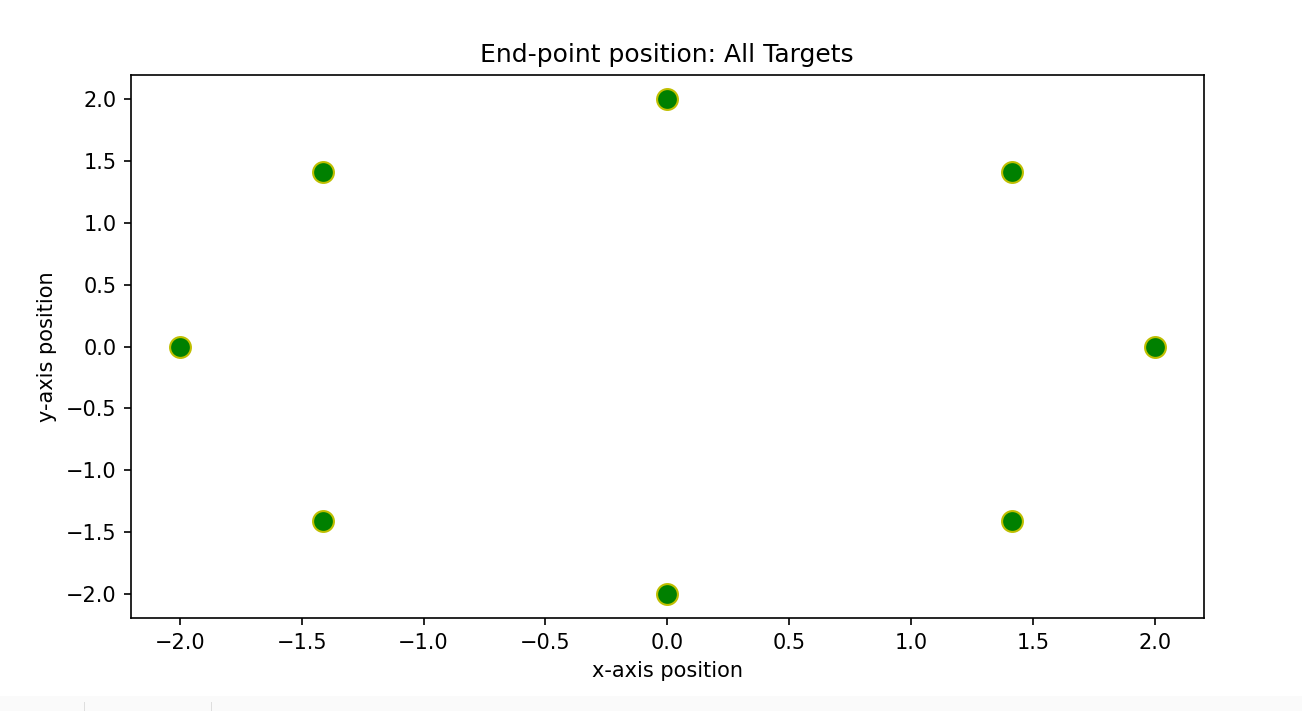
\includegraphics[width=0.55\textwidth]{points}
	\end{figure}
	
Tarea a realizar:
	\begin{enumerate}
		\item Situar el cursor sobre el target de referencia (en el centro).
		\item El target de referencia desaparecerá y en su lugar aparecerá otro target situado en una de las 8 posiciones de la imagen. El sujeto debe situar el cursor sobre dicho target dentro del tiempo disponible para hacerlo.
		\item Al situar el cursor sobre el target objetivo el punto desaparecerá y volverá a aparecer el target de referencia. Lo mismo ocurrirá si se acaba el tiempo y el sujeto no sitúa el cursor sobre el target (en este caso habrá un sonido de amonestación).
	\end{enumerate}	
\begin{itemize}
	\item Las trayectorias que guardaremos serán las del target de referencia al target objetivo.
\end{itemize}	
\end{frame}

\begin{frame}
	\frametitle{Fases del experimento}

	\begin{enumerate}
		\item \textbf{Fase libre}: no hay ningún target y el sujeto es libre de mover el cursor como quiera. 
		\item \textbf{Primera fase}: sin ninguna fuerza y mostrando el cursor.
		\item \textbf{Segunda fase}: con fuerza (en el eje x, sentido negativo) y mostrando el cursor.
		\item \textbf{Tercera fase}: sin fuerza y sin mostrar el cursor.
		\item \textbf{Cuarta fase}: con fuerza y sin mostrar el cursor.
	\end{enumerate}	
	\begin{itemize}
		\item En cada una de las fases se harán 80 repeticiones de la tarea definida antes.
	\end{itemize}
\end{frame}
\begin{frame}
	\frametitle{Parámetros definidos en la Fase de Prueba}
	
	\begin{itemize}
		\item Número de repeticiones por fase. 
		\item Tiempo para la realización del experimento.
		\item Número y disposición de los puntos objetivo.
		\item Puntos en orden o de forma aleatoria.
	\end{itemize}	
\begin{figure}
	\centering
	\subfloat{
		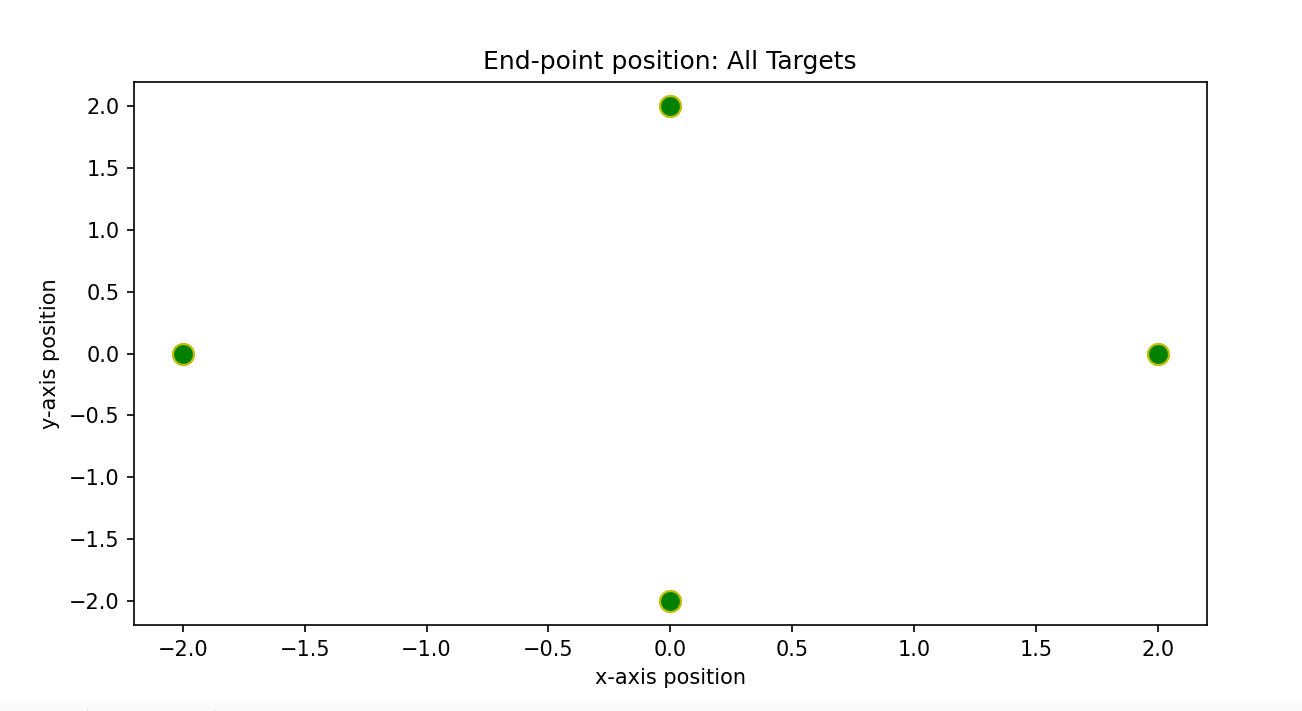
\includegraphics[width=0.5\textwidth]{points-4}}
	\subfloat{
		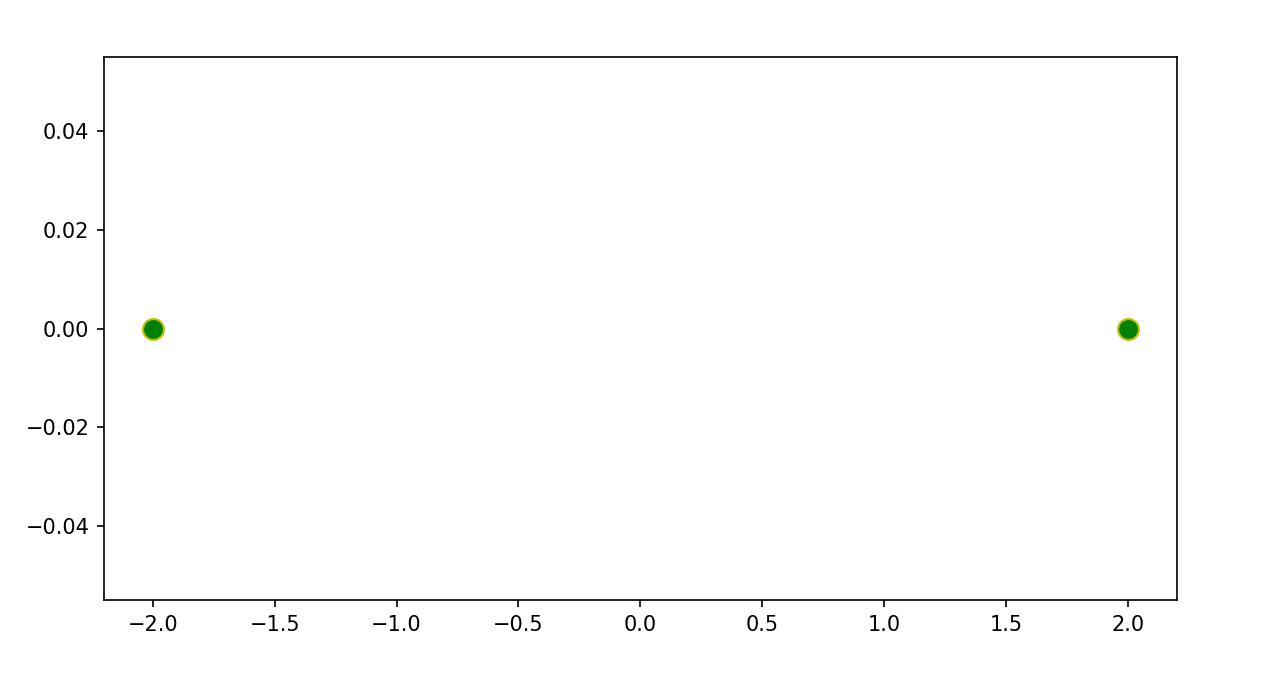
\includegraphics[width=0.5\textwidth]{puntos2}}
\end{figure}

\end{frame}

\subsection{Desarrollo de la aplicación}
\begin{frame}
	\frametitle{Desarrollo}
		\begin{itemize}
		\item Bucle gráfico: 30 Hz.
		\item Servoloop: 1000 Hz, máxima prioridad.
	\end{itemize}
	\begin{figure}
	\centering
	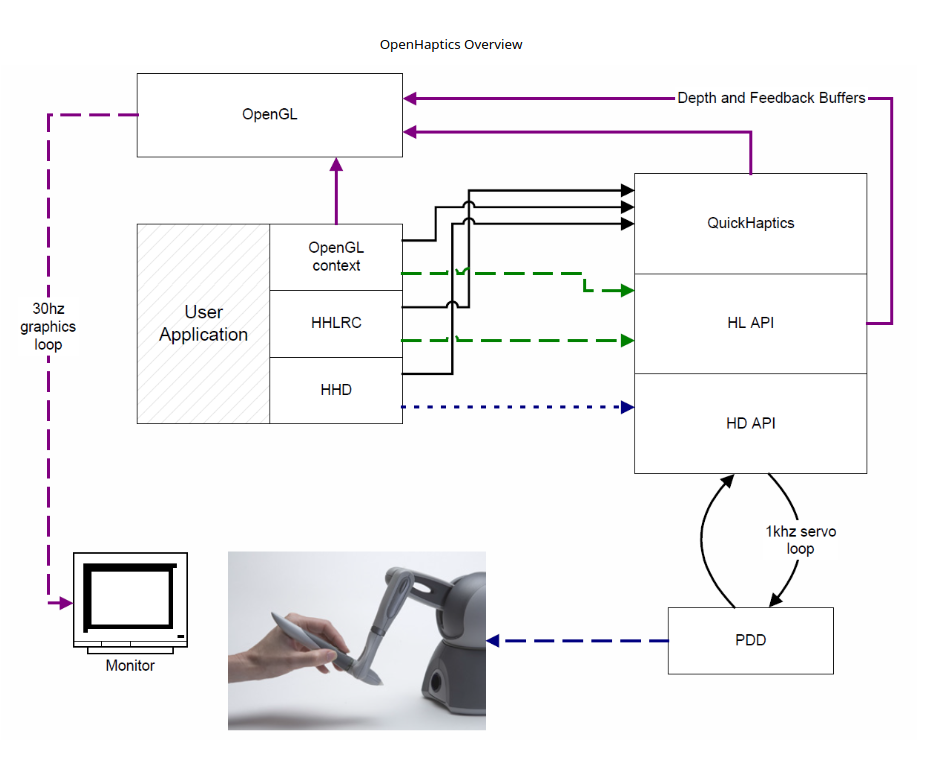
\includegraphics[width=0.8\textwidth]{estructura}
	\end{figure}

\end{frame}
\begin{frame}
	\frametitle{Desarrollo}
	\begin{itemize}
		\item \textbf{Callbacks}
		\begin{itemize}
			\item Síncronas o asíncronas
			\item Con return code DONE o CONTINUE
			\item Algunos ejemplos:
			\begin{itemize}
				\item beginUpdateCallback (asíncrona, continue)
				\item forceCallback (asíncrona, continue)
				\item actionInitialized (asíncrona, done)
				\item actionFinished (asíncrona, done)
				\item setDeviceTransformationCallback (síncrona, done)
			\end{itemize}
		\end{itemize}

	\end{itemize}
	
\end{frame}
\begin{frame}
	\frametitle{Desarrollo}
		\begin{figure}
		\centering
		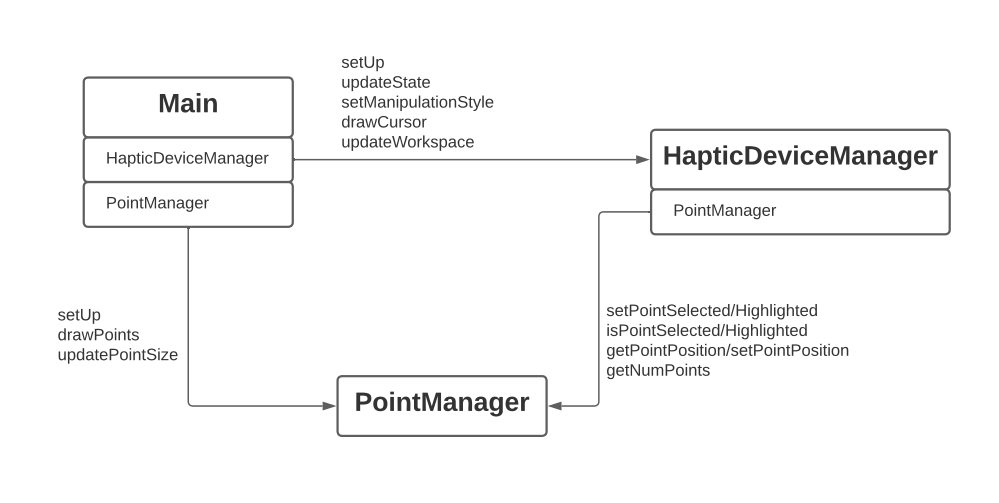
\includegraphics[width=\textwidth]{diagrama}
	\end{figure}
	
\end{frame}
\section{Resultados}
\subsection{Obtención de resultados}
\begin{frame}
	\frametitle{Muestra de sujetos elegidos}
\begin{table}[H]
	\centering
	\begin{tabular}{l l | l l}
		\multicolumn{2}{ c }{Fase 1} & \multicolumn{2}{ c }{Fase 2} \\ 
		Sexo & Edad & Sexo & Edad\\\hline 
		
		Mujer & 23 & Mujer & 20 \\
		Mujer & 24  & Mujer & 22\\
		Hombre & 53 & Hombre & 50\\
		Mujer & 52 & Hombre & 60 \\
		Hombre & 62  & Mujer & 60\\\
		Mujer & 60 \\
		Hombre & 90 \\
		Mujer & 90 \\
	\end{tabular} 
\end{table}
	
\end{frame}
\begin{frame}
	\frametitle{Muestra de sujetos elegidos}

		\begin{itemize}
			\item Sujeto 1: Mujer, 20 años, en orden
			\item Sujeto 2: Mujer, 22 años, aleatorio
			\item Sujeto 3: Mujer, 60 años, aleatorio
			\item Sujeto 4: Hombre, 50 años, en orden
			\item Sujeto 5: Hombre, 60 años, en orden
		\end{itemize}

	
\end{frame}
\begin{frame}
	\frametitle{Aplicación}
	
	\begin{figure}
		\centering
	
			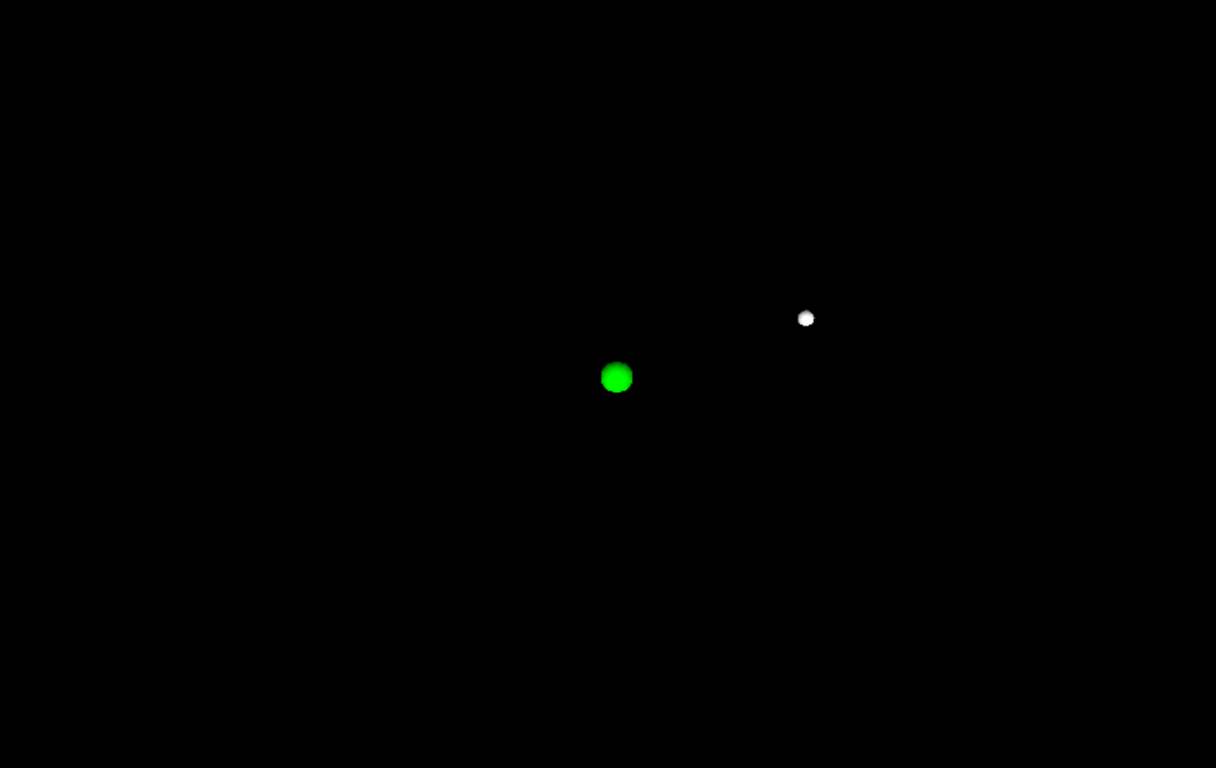
\includegraphics[width=0.5\textwidth]{cursor}
	
	\end{figure}
	\begin{figure}
	\centering
	
	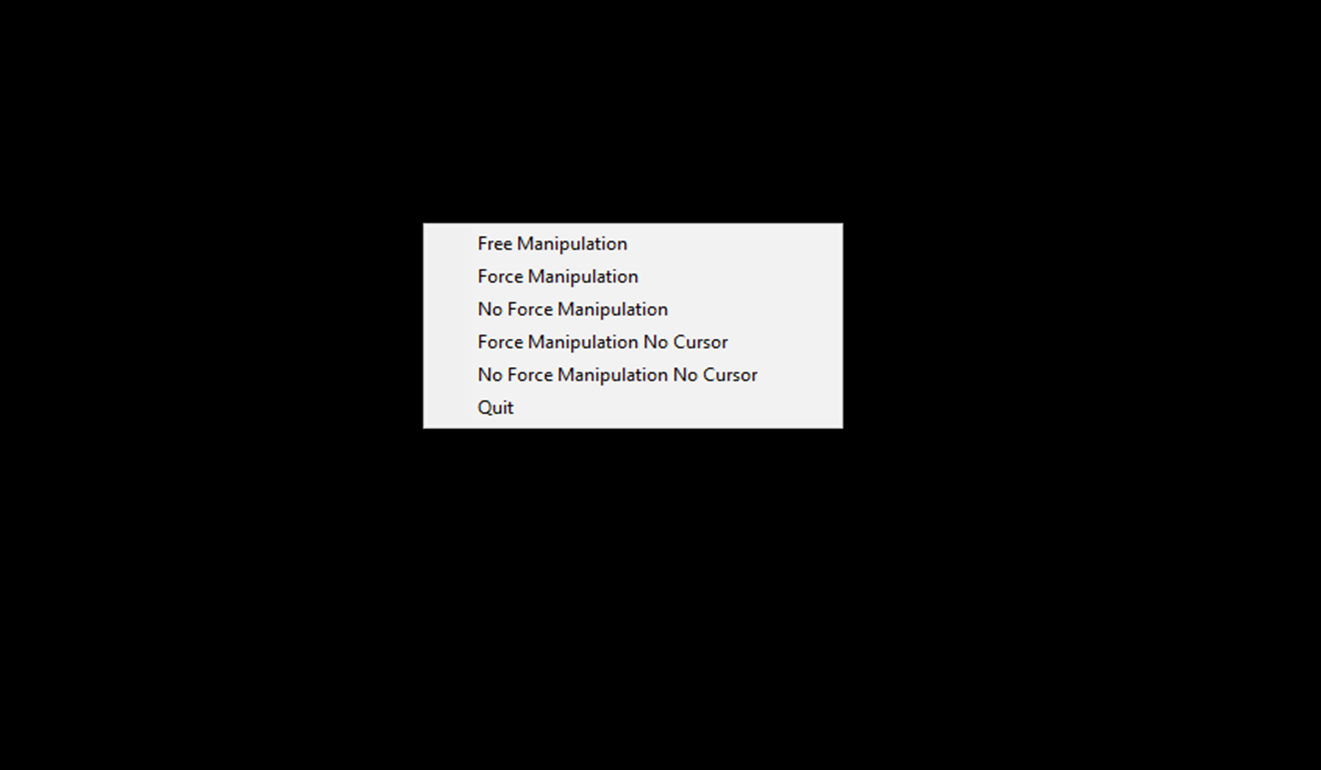
\includegraphics[width=0.6\textwidth]{menu}

\end{figure}
\end{frame}

\section{Conclusiones}
\end{document}
